%%%%%%%%%%%%%%%%%%%%
% - - - - - - - - PART JOAN - - - - - - - - - 
%%%%%%%%%%%%%%%%%%%%
\section{First Placement}
The aim of this part is to explain the first placement of the constellation. It is divided in two parts. The first one is intended to give a first approach to the logistics involved in the first placement, whereas the second one is focused on the maneuver required so as to deploy the satellites into orbit. 

\subsection{First Placement logistics}
Gantt charts provided by Rocketlab USA:

\begin{figure}[H]
\centering 
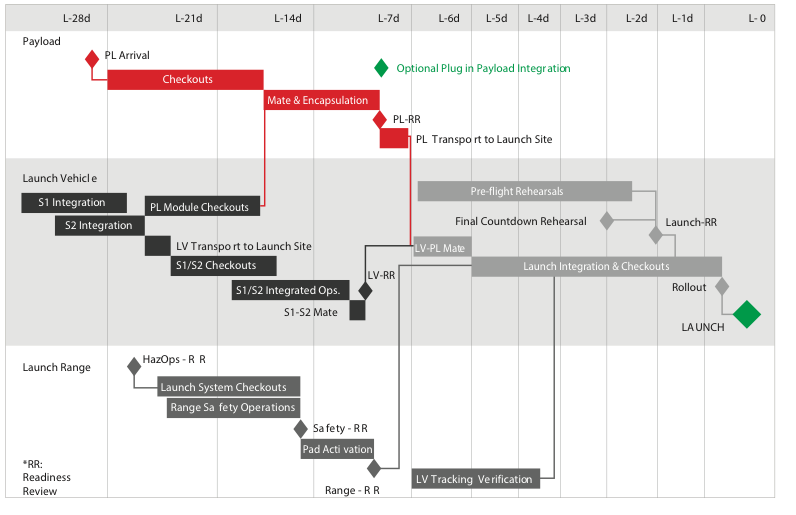
\includegraphics[scale=0.7]{./sections/Constellation_Deployment/S4-First_Placement/Images_S4/Picture_1_S4.png} 
\caption{Launch Range Operations Flow/Schedule}
\label{fig:gantt1}
\end{figure}

\begin{figure}[H]
\centering 
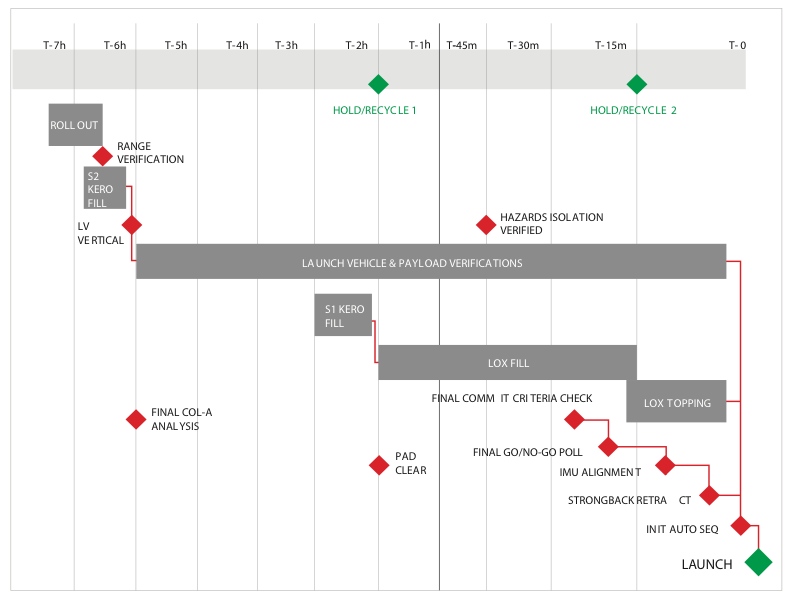
\includegraphics[scale=0.7]{./sections/Constellation_Deployment/S4-First_Placement/Images_S4/Picture_2_S4.png} 
\caption{Countdown Operations Flow}
\label{fig:gantt2}
\end{figure}

%%%%%%%%%%%%%%%%%%%%%%%%%%%%%%%%%%%%%%%%
% - - - - - - - - - PART ROGER - - - - - - - - - - 
%%%%%%%%%%%%%%%%%%%%%%%%%%%%%%%%%%%%%%%%
\subsection{1st Placement In-Orbit Injection Maneuver}
In a more schematic way, the procedure goes as follows:

\begin{enumerate}
\item The rocket goes through the procedure designed by Rocketlab USA to get to the destination orbit. The approximate trajectory during this stage is represented in \ref{orbit1}.Right after entering into the destination orbit, the first satellite is deployed into it as seen in \ref{orbit1} represented with a red dot.
\item Once the latter is completed, the rocket's engine gives it the necessary $\Delta V$ in order to get to the elliptical spacing orbit. In \ref{orbit2} half a revolution of the rocket is represented along with the orbit of the first deployed satellite at the same point in time.
\item After one full revolution of the rocket in the elliptical orbit, the first satellite will have left the right phase spacing with respect to the rocket. At this point the rocket's engine gives the same $\Delta V$ as in step 2 but negative. This will cause it to enter again into the circular orbit of the satellites. At this point the rocket deploys the second satellite as shown in \ref{orbit3}. Right after this deployment the rocket enters into the elliptical orbit again.
\item \ref{orbit4} represents again half a revolution of the rocket in the elliptical orbit along with the deployed satellites so far.
\item Finally, the rocket reduces its velocity again to enter into the circular destination orbit in order to deploy the third satellite (\ref{orbit5}).
\item This aforementioned procedure is iterated until the orbital plane is full.
\newline\newline
\end{enumerate}

\begin{figure}[H]
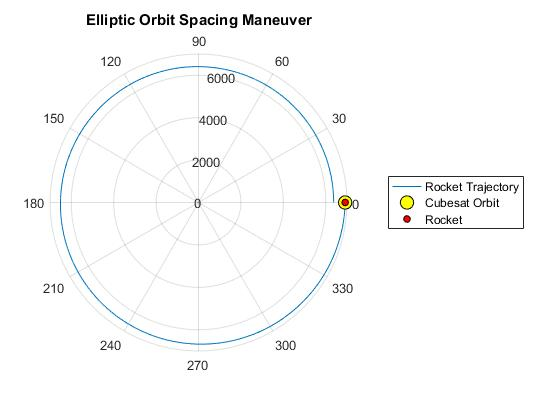
\includegraphics[scale=0.7]{./sections/Constellation_Deployment/S4-First_Placement/Images_S4/Picture_3_S4.jpg}
\caption{Rocket's trajectory from lift-off to final orbit.}
\label{orbit1}
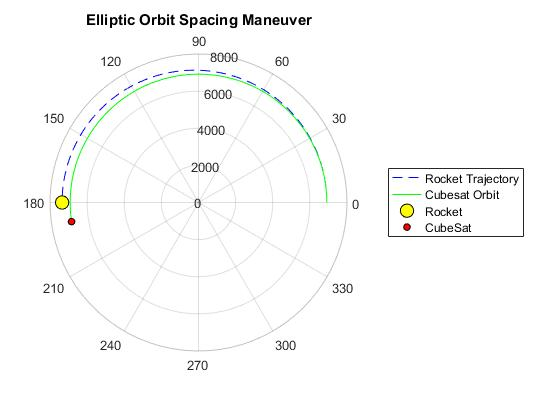
\includegraphics[scale=0.7]{./sections/Constellation_Deployment/S4-First_Placement/Images_S4/Picture_4_S4.jpg}
\caption{Half of a revolution of the rocket in the elliptical spacing orbit.}
\label{orbit2}
\end{figure}

\begin{figure}[H]
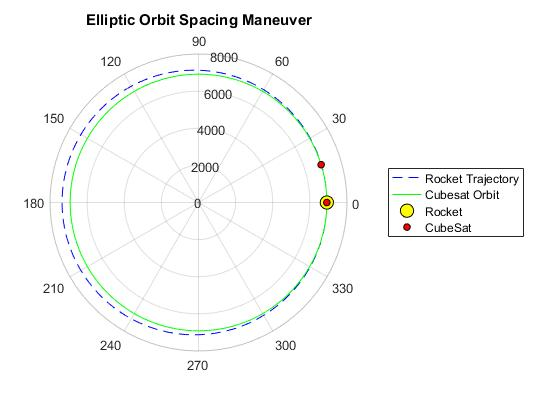
\includegraphics[scale=0.7]{./sections/Constellation_Deployment/S4-First_Placement/Images_S4/Picture_5_S4.jpg}
\caption{Deployment of the second satellite.}
\label{orbit3}
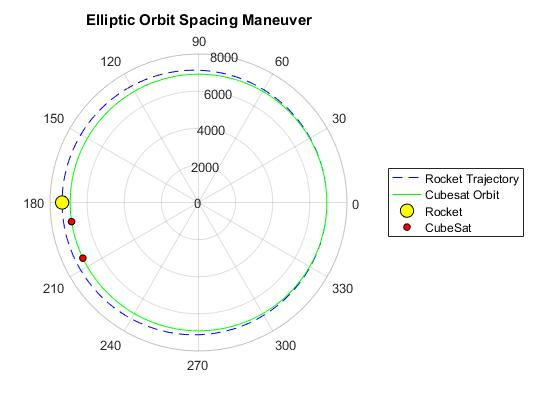
\includegraphics[scale=0.7]{./sections/Constellation_Deployment/S4-First_Placement/Images_S4/Picture_6_S4.jpg}
\caption{Half of a revolution of the rocket after the deployment of the second satellite.}
\label{orbit4}
\end{figure}

\begin{figure}[H]
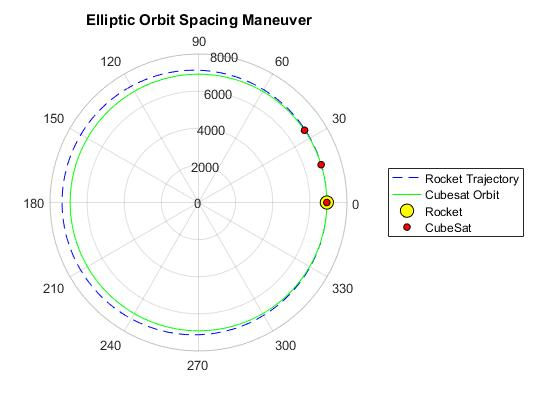
\includegraphics[scale=0.7]{./sections/Constellation_Deployment/S4-First_Placement/Images_S4/Picture_7_S4.jpg}
\caption{Deployment of the third satellite.}
\label{orbit5}
\end{figure}

\subsection{Orbit Parameters Calculation}
\begin{center}
$V_s = \sqrt{\frac{GM_t}{R_t\,+\,h}} $
\newline\newline
$T_s = \frac{2\pi(R_t\,+\,h)}{V_s}$\newline
\end{center}

Where $R_t$ and h are Earth's radius and height above Earth's surface respectively. For $h = 542 \,km$, the values obtained are $V_s = 7,589.6 \,m/s$ and $T_s = 5,723.1 \,s$. Let's call the spacing between satellites $\theta = \frac{360^\circ}{21} = 17.14^\circ$ and $R = R_t \,+ \,h$. Using these values it is possible to compute the period of the elliptical orbit, $T_r$, along with the rest of the parameters:

\begin{center}
$T_r = T_s\,+\,\frac{\theta R}{V_s} = 5,995.6\,s$

$a = (\frac{T_r}{2\pi}^2GM_t)^\frac{1}{3}=7,130.8\,km$

$R_1 = R;\;\;\;R_2=2a\,-\,R_1$

$c = a\,-\,R_1;\;\;\;b = \sqrt{a^2\,-c^2}$

$\epsilon = \sqrt{1\,-\,\frac{b^2}{a^2}}=0.0305$

$\Delta V = \sqrt{\frac{GM_t}{R1}}\,(\sqrt{\frac{2R_2}{R1\,+\,R2}}-1)=115.01\,m/s$

\end{center}

\subsubsection{Plane Order}
The aim of this section is to describe the order in which all of the 9 planes are put into orbit. The fact that establishes one path or another is the fact that satellites can only communicate with neighbours, that is, one satellite can only communicate with its neighbours from the same plane and the neighbours from the neighbour planes.

When it comes to the order in which the planes are put into orbit, there are two main ways that come to mind. The first one is putting the planes consecutively into orbit. The second one is to put the planes into orbit leaving space between them for future planes. For example plane number one is put into orbit. The second plane to be put into orbit leaves space for one plane in between them. Then the third leaves space for one plane from the second, and so on. Leaving more space than for one plane could also be an option.

On the one hand, when using the first way the satellites from each plane could communicate with the ones from their neighbourhood. Therefore the range of communication would start being narrower but as new planes are put into orbit, the range would become wider. For instance, when three planes are already working, a given satellite form a customer could communicate with satellites that are at the other side of the planet in a determined range given by the width of signal that those three orbital planes could cover. When new planes are put into orbit this width becomes bigger up until the full globe is covered. Of course the main drawback of using this consecutive way of putting planes into orbit would be the long time of inactivity right at the beginning when few planes are working.

On the other hand, when using the second described way, the satellites can't communicate with other satellites from neighbour planes but the time of inactivity for customer's satellites would be less as a gap between planes is left for future ones. Nevertheless, this kind of configuration has a huge drawback and it's that when a satellite communicates with one given plane, this one can only communicate with other satellites that are in the range of signal emission of that given plane. This is due to the fact that as neighbour planes are further apart they can't communicate with each other and therefore the range of communication is affected.

Having pointed out all of the advantages and drawbacks of each configuration it is time to choose and it all comes down to Astrea's preferences. The configuration that fulfills these preferences for the most part is the consecutive one. It allows the satellites to communicate in a broader range as the constellation grows and progressively conquer the sky.